\documentclass[class=article, crop=false, 12pt,a4paper]{standalone}
\usepackage{enumitem}
\usepackage{multicol}
\usepackage{etoolbox}
\AtBeginEnvironment{quote}{\singlespacing\small}
\usepackage{setspace}
\onehalfspacing
\usepackage{graphicx}
\usepackage{float}
\usepackage{amsmath}
\usepackage{amssymb}
\numberwithin{equation}{section}
\usepackage{mathtools}
\usepackage{siunitx}
\DeclareSIUnit\rev{rev}
\sisetup{detect-all}
\begin{document}
\title{Energy balance lab report}
\author{Hasha Dar}
\date{February 4, 2020}
\maketitle
\tableofcontents
\newpage
\section{Lab data}
\subsection{1 bar}
\begin{multicols}{2}
  \begin{itemize}[noitemsep]
    \item \(T_0\) = 25 \si{\celsius}
    \item \(T_1\) = 23 \si{\celsius}
    \item \(P_0\) = 1 \si{bar}
    \item \(P_1\) = 0.05 \si{bar}
    \item \(P_2\) = 1 \si{\bar}
    \item \(V_{in}\) = 285 \si{\liter\per\minute}
    \item \(N\) = 1430 \si{\rev\per\second}
    \item \(F\) = 1.5 \si{\kg}
    \item \(\dot{W}_{el}\) = 1150 \si{\watt}
  \end{itemize}
\end{multicols}
\subsubsection{\(T_2\) readings} 
\begin{table}
  \centering
    \begin{tabular}{|c|c|}
      \hline
      Time (\si{\minute}) & \(T_2\) (degrees C)\\
      \hline
      0 & 95\\
      1 & 98\\
      2 & 101\\
      3 & 104\\
      4 & 106\\
      5 & 108\\
      6 & 110\\
      7 & 112\\
      8 & 114\\
      9 & 116\\
      10 & 118\\
      11 & 119\\
      12 & 121\\
      13 & 122\\
      14 & 124\\
      15 & 125\\
      16 & 127\\
      17 & 128\\
      18 & 130\\
      19 & 131\\
      20 & 131\\
      \hline
    \end{tabular}
  \caption{\(T_2\) readings from apparatus with 1 bar compressor}
  \label{table:1}
\end{table}
\subsection{0.6 bar}
\begin{multicols}{2}
  \begin{itemize}[noitemsep]
    \item \(T_0\) = 25 \si{\celsius}
    \item \(T_1\) = 24 \si{\celsius}
    \item \(P_0\) = 1 \si{\bar}
    \item \(P_1\) = 0.06 \si{\bar}
    \item \(P_2\) = 1 \si{\bar}
    \item \(V_{in}\) = 310 \si{\liter\per\minute}
    \item \(N\) = 1445 \si{\rev\per\second}
    \item \(F\) = 1.5 \si{\kilogram}
    \item \(\dot{W}_{el}\) = 1000 \si{\watt}
  \end{itemize}
\end{multicols}
\subsubsection{\(T_2\) readings}
\begin{table}
  \centering
    \begin{tabular}{|c|c|}
      \hline
      Time (\si{\minute}) & \(T_2\) (degrees C)\\
      \hline  
      0 & 63\\
      1 & 68\\
      2 & 71\\
      3 & 74\\
      4 & 77\\
      5 & 79\\
      6 & 81\\
      7 & 84\\
      8 & 86\\
      9 & 88\\
      10 & 89\\
      11 & 91\\
      12 & 92\\
      13 & 94\\
      14 & 95\\
      15 & 97\\
      16 & 98\\
      17 & 99\\
      18 & 101\\
      19 & 102\\
      20 & 103\\
      \hline
    \end{tabular}
  \caption{\(T_2\) readings from apparatus with 0.6 bar compressor}
  \label{table:2}
\end{table}
\subsection{0.3 bar}
\begin{multicols}{2}
  \begin{itemize}[noitemsep]
    \item \(T_0\) = 25 \si{\celsius}
    \item \(T_1\) = 25 \si{\celsius}
    \item \(P_0\) = 1 \si{\bar}
    \item \(P_1\) = 0.08 \si{\bar}
    \item \(P_2\) = 1 \si{\bar}
    \item \(V_{in}\) = 320 \si{\liter\per\minute}
    \item \(N\) = 1459 \si{\rev\per\second}
    \item \(F\) = 1.5 \si{\kilogram}
    \item \(\dot{W}_{el}\) = 850 \si{\watt}
  \end{itemize}
\end{multicols}
\subsubsection{\(T_2\) readings}
\begin{table}
  \centering
    \begin{tabular}{|c|c|}
      \hline
      Time (\si{\minute}) & \(T_2\) (degrees C)\\
      \hline  
      0 & 52\\
      1 & 55\\
      2 & 58\\
      3 & 60\\
      4 & 62\\
      5 & 63\\
      6 & 65\\
      7 & 67\\
      8 & 68\\
      9 & 69\\
      10 & 70\\
      11 & 71\\
      12 & 72\\
      13 & 73\\
      14 & 74\\
      15 & 75\\
      16 & 76\\
      17 & 76\\
      18 & 77\\
      19 & 78\\
      20 & 78\\
      \hline
    \end{tabular}
  \caption{\(T_2\) readings from apparatus with 0.3 bar compressor}
  \label{table:3}
\end{table}
\section{Experiment 1 calculations}
All the calculations completed below were done with data from the 1 bar experiment.
\subsection{Volumetric flow rate}
The formula for the volumetric flow rate is:
\begin{equation}
  \dot{V} = \frac{V_{in}}{60 \times 10^3} \ \si{\meter\cubed\per\second}
  \label{volflowrate}
\end{equation}
Thus, our volumetric flow rate (using equation \ref{volflowrate}) is:
\begin{equation} 
  \dot{V} = \frac{285}{60\times 10^3} = \frac{19}{4000} = 4.75 \times 10^{-3} \ \si{\meter\cubed\per\second} \ (3\textrm{sf})
\end{equation}
\subsection{Mass flow rate}
The specific volume through flowmeter is given by the following equation
\begin{equation}
  v_0 = \frac{RT_0}{P_0} \ \si{\meter\cubed\per\kg} \textrm{ where \(R = 0.287 \ \si{\kilo\joule\per\kg\per\kelvin}\)}
  \label{specvol}
\end{equation}
The mass flow rate is given by the following equation:
\begin{equation}
  \dot{m} = \frac{\dot{V}}{v_0} \ \si{\kg\per\second}
  \label{massflowrate}
\end{equation}
Calculating the specific volume (\ref{specvol}) and inputting the volume flow rate calculated previously (\ref{volflowrate}) our mass flow rate is:
\begin{align} 
  v_0 &= \frac{0.287 \cdot (25+273.15)}{100} = 0.856 \ \si{\kg\per\second} \ (3\textrm{sf})  \\
  \dot{m} &= \frac{4.75 \times 10^{-3}}{0.856} = 5.55 \times 10^{-3} \ \si{\kg\per\second} \ (3\textrm{sf}) 
\end{align}
\subsection{Energy added to air by compressor}
The equation to calculate the energy added to air by compressor is:
\begin{equation}
  \dot{H}_c = \dot{m}c_P(T_2-T_1) \ \si{\watt} \textrm{ where \(c_P\) is 1005 \si{\kilo\joule\kg\per\kelvin}}
  \label{energyaddaircompressor}
\end{equation}
Inputting the variables into equation \ref{energyaddaircompressor}, we get: 
\begin{equation} 
  \dot{H}_c = 5.55 \times 10^{-3} \times 1005 \times (131-23) = 602.296 \ \si{\watt} \ (3\textrm{dp}) 
\end{equation}
\subsection{Power out of motor}
The equation for the power out of the motor is:
\begin{equation}
  \dot{W}_{m} = \frac{19.62NFL\pi}{60} \ \si{\watt}
  \label{motorpower}
\end{equation}
Thus, our motor power is:
\begin{equation} 
  \dot{W}_{m} = \frac{19.62 \times 1430 \times 1.5 \times 0.2 \times \pi}{60} = 440.712 \ \si{\watt} \ (3\textrm{dp})
\end{equation}
\subsection{Heat losses in the compressor}
The equation for the heat emitted from the compressor is:
\begin{equation}
  \dot{Q}_c = \dot{W}_m - \dot{H}_c \ \si{\watt}
  \label{heatlosscompressor}
\end{equation}
Thus, our motor heat losses are:
\begin{equation} 
  \dot{Q}_c = 440.712 - 602.296 = -161.685 \ \si{\watt} \ (3\textrm{dp}) 
\end{equation}
\section{Experiment 1 discussion}
\subsection{Outlet temperature against time plot}
Importing the data into MATLAB, I plotted the data on a graph.
\begin{figure}
  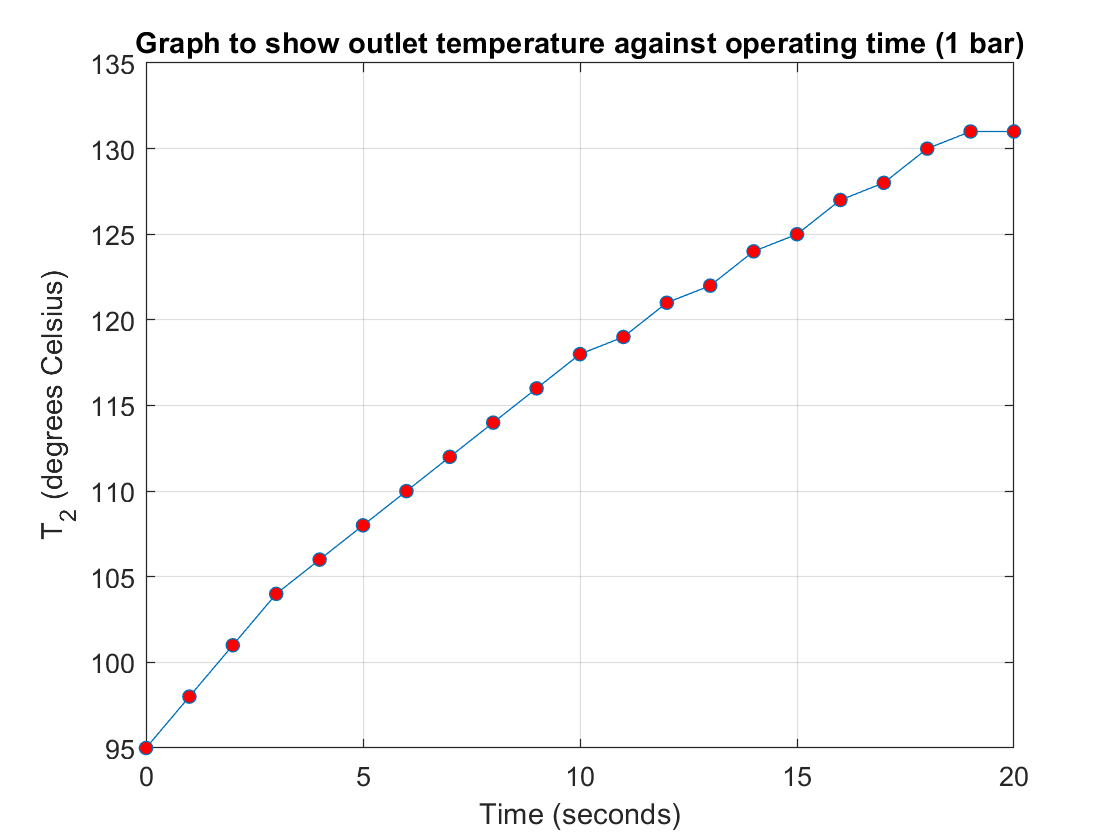
\includegraphics[width = 0.9 \textwidth]{./img/T21vsTimeGraph}
  \caption{Plot of \(T_2\) against the operating time of the apparatus (1 bar)}
  \label{ref:T21vsTime1bar}
\end{figure}
\begin{figure}
  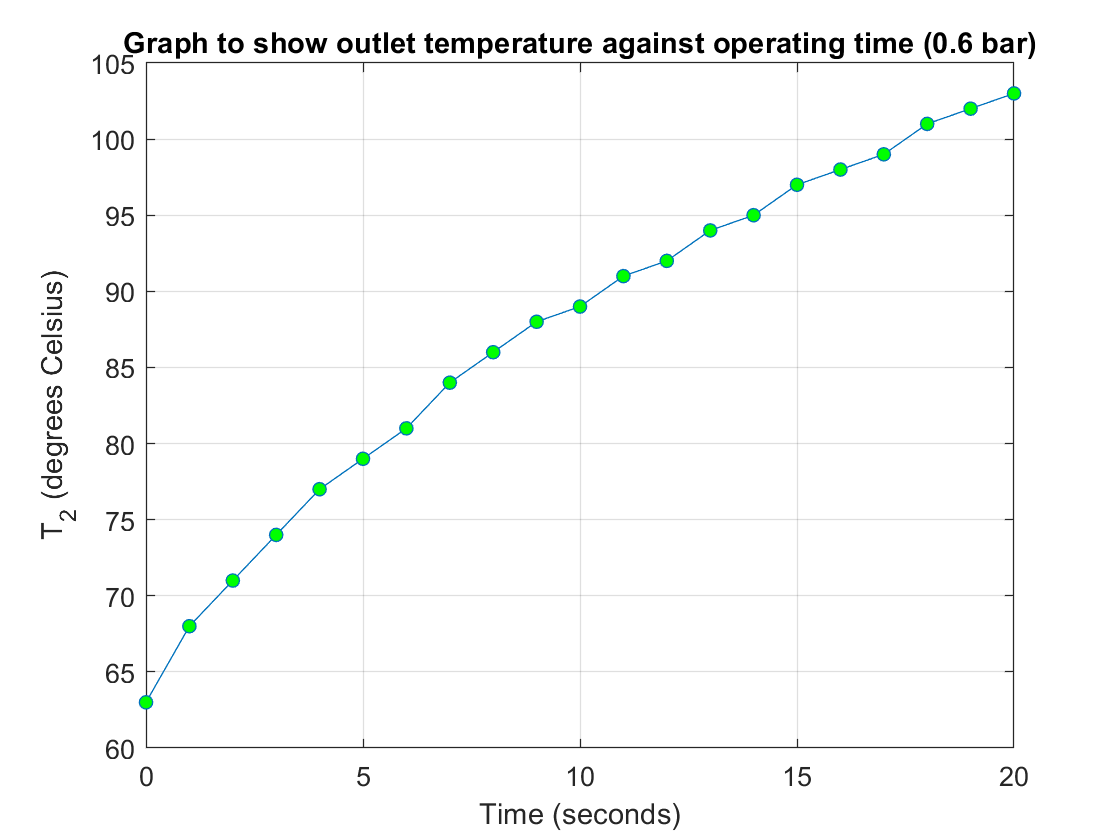
\includegraphics[width = 0.9 \textwidth]{./img/T206vsTimeGraph}
  \caption{Plot of \(T_2\) against the operating time of the apparatus (0.6 bar)}
  \label{ref:T206vsTime1bar}
\end{figure}
\begin{figure}
  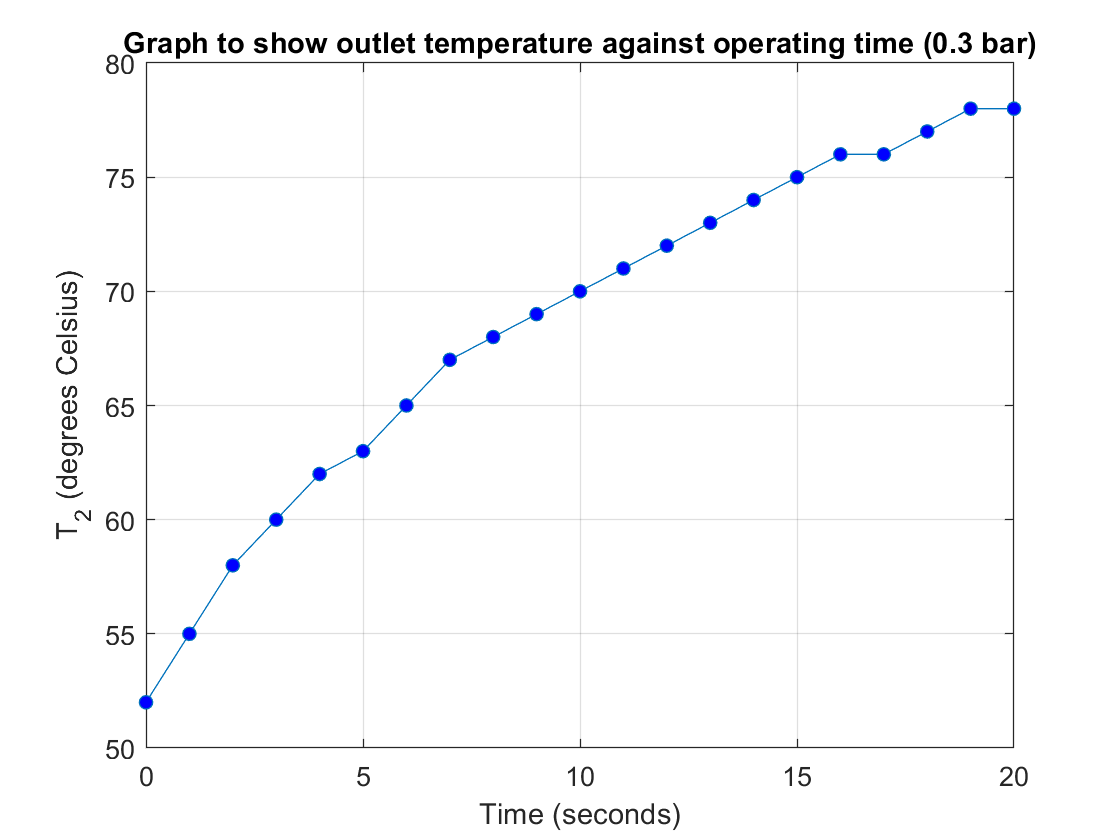
\includegraphics[width = 0.9 \textwidth]{./img/T203vsTimeGraph}
  \caption{Plot of \(T_2\) against the operating time of the apparatus (0.3 bar)}
  \label{ref:T203vsTime1bar}
\end{figure}
\subsection{Why does the graph have this shape?}
\subsection{What happens to the system's energy input as it heats up?}
\subsection{How does the energy lost as heat compare to:}
\subsubsection{The work input to the compressor?}
\subsubsection{The heat added to the air?}
\section{Experiment 2 calculations}
\subsection{Specific volume of air at atmosphere and the inlet and outlet of compressor}
We can calculate the specific volumes at atmosphere, before and after the compressor using equation \ref{specvol}, which is shown below.
\begin{equation}
  v_0 = \frac{RT_0}{P_0} \ (\si{\meter\cubed\per\kg}) \textrm{ where \(R = 0.287 \ \si{\kilo\joule\per\kg\per\kelvin}\)}
  \tag{\ref{specvol}}
\end{equation}
Thus, at atmosphere, our specific volume of air is:
\begin{equation} 
  v_0 = \frac{0.287 \times (25+273.15)}{100} = 0.856 \ \si{\meter\cubed\per\kg} \ (3\textrm{sf}) 
\end{equation}
The temperature is constant before the compressor and \(T_2\) approaches a constant value after some time, hence we can use a formula for specific volume where T is constant:
\begin{equation}
  v_1 = v_0 \times \left( \frac{P_0}{P_0 - P_1} \right) \ \si{\meter\cubed\per\kg}
  \label{constpspecvol}
\end{equation}
Using equation \ref{constpspecvol}, the specific volume before the compressor is:
\begin{align} 
  v_1 &= 0.856 \times \left( \frac{100}{100-5} \right) = \frac{428}{475} = 0.901 \ \si{\meter\cubed\per\kg} \ (3\textrm{sf}) \textrm{ (1 bar)} \\
  v_1 &= 0.856 \times \left( \frac{100}{100-6} \right) = \frac{214}{235} = 0.911 \ \si{\meter\cubed\per\kg} \ (3\textrm{sf}) \textrm{ (0.6 bar)} \\
  v_1 &= 0.856 \times \left( \frac{100}{100-8} \right) = \frac{107}{115} = 0.930 \ \si{\meter\cubed\per\kg} \ (3\textrm{sf}) \textrm{ (0.3 bar)} 
\end{align}
Using equation \ref{constpspecvol}, the specific volume after the compressor is:
\begin{equation} v_2 = 0.856 \times \left( \frac{100}{100+100} \right) = \frac{107}{115} = 0.428 \ \si{\meter\cubed\per\kg} \ (3\textrm{sf}) \textrm{ (1, 0.6, 0.3 bar)} \end{equation}
\subsection{Volumetric flow rate of air}
Using equation \ref{volflowrate} we can calculate the volumetric flow rate of air.
\begin{align}
  \dot{V} &= \frac{V_{in}}{60 \times 10^3} \ \si{\meter\cubed\per\second} \tag{\ref{volflowrate}}\\
  \dot{V} = \frac{285}{60\times 10^3} = \frac{19}{4000} &= 4.75 \times 10^{-3} \ \si{\meter\cubed\per\second} \ (3\textrm{sf}) \ \textrm{ (1 bar)}\\
  \dot{V} = \frac{310}{60\times 10^3} = \frac{31}{6000} &= 5.17 \times 10^{-3} \ \si{\meter\cubed\per\second} \ (3\textrm{sf}) \ \textrm{ (0.6 bar)}\\
  \dot{V} = \frac{320}{60\times 10^3} = \frac{2}{375} &= 5.33 \times 10^{-3} \ \si{\meter\cubed\per\second} \ (3\textrm{sf}) \ \textrm{ (0.3 bar)}
\end{align}
\subsection{Mass flow rate of air}
The mass flow rate of air can be calculated using equation \ref{massflowrate}.
\begin{equation}
  \dot{m} = \frac{\dot{V}}{v_0} \ \si{\kg\per\second}
  \tag{\ref{massflowrate}}
\end{equation}
Calculating the specific volume (\ref{specvol}) and inputting the volume flow rate (\ref{volflowrate}) our mass flow rate is:
\begin{align}
  v_0 &= \frac{0.287 \cdot (25+273.15)}{100} = 0.856 \ \si{\kg\per\second} \ (3\textrm{sf})  \\
  \dot{m} &= \frac{4.75 \times 10^{-3}}{0.856} = 5.55 \times 10^{-3} \ \si{\kg\per\second} \ (3\textrm{sf}) \textrm{ (1 bar)} \\
  \dot{m} &= \frac{5.17 \times 10^{-3}}{0.856} = 6.04 \times 10^{-3} \ \si{\kg\per\second} \ (3\textrm{sf}) \textrm{ (0.6 bar)} \\
  \dot{m} &= \frac{5.33 \times 10^{-3}}{0.856} = 6.23 \times 10^{-3} \ \si{\kg\per\second} \ (3\textrm{sf}) \textrm{ (0.3 bar)}
\end{align}
\subsection{Theoretical mass flow rate of air}
The compressors swept volume is \(V_{comp} = 2.67 \times 10^{-4}\), hence we can calculate the theoretical mass flow rate using equation \ref{massflowrate}.
\begin{align}
  \dot{m} &= \frac{\dot{V}_{comp} \times N}{60 \times v_0} \ \si{\kg\per\second} \tag{\ref{massflowrate}}\\
  \dot{m} = \frac{2.67 \times 10^{-4} \times 1430}{60 \times 0.856} &= 7.43 \times 10^{-3} \ \si{\kg\per\second} \ (3\textrm{sf}) \textrm{ (1 bar)}\\
  \dot{m} = \frac{2.67 \times 10^{-4} \times 1445}{60 \times 0.856} &= 7.51 \times 10^{-3} \ \si{\kg\per\second} \ (3\textrm{sf}) \textrm{ (0.6 bar)}\\
  \dot{m} = \frac{2.67 \times 10^{-4} \times 1459}{60 \times 0.856} &= 7.58 \times 10^{-3} \ \si{\kg\per\second} \ (3\textrm{sf}) \textrm{ (0.3 bar)}
\end{align}
\subsection{Pressure ratio}
The pressure ratio is given by the following equation:
\begin{equation}
  r_P = \frac{\textrm{Pressure out}}{\textrm{Pressure in}} = \frac{P_0 + P_2}{P_0-P_1}
\end{equation}
Thus, our pressure ratios are:
\begin{align}
  r_P = \frac{100000 + 100000}{100000-5000} = \frac{40}{19} &= 2.11 \ (3\textrm{sf}) \ (1 \textrm{ bar})\\
  r_P = \frac{100000 + 100000}{100000-6000} = \frac{100}{47} &= 2.13 \ (3\textrm{sf}) \ (0.6 \textrm{ bar})\\
  r_P = \frac{100000 + 100000}{100000-8000} = \frac{50}{23} &= 2.17 \ (3\textrm{sf}) \ (0.3 \textrm{ bar})
\end{align}
\subsection{Motor power}
The equation for motor power is already given in equation \ref{motorpower}.
\begin{equation}
  \dot{W}_{m} = \frac{19.62NFL\pi}{60} \ \si{\watt}
  \tag{\ref{motorpower}}
\end{equation}
Thus, our motor powers are:
\begin{align}
  \dot{W}_{m} = \frac{19.62(1430)(1.5)(0.2)\pi}{60} &= 440.712\ \si{\watt} \ (3\textrm{dp}) \ (1 \textrm{ bar})\\
  \dot{W}_{m} = \frac{19.62(1445)(1.5)(0.2)\pi}{60} &= 445.335\ \si{\watt} \ (3\textrm{dp}) \ (0.6 \textrm{ bar})\\
  \dot{W}_{m} = \frac{19.62(1459)(1.5)(0.2)\pi}{60} &= 449.650\ \si{\watt} \ (3\textrm{dp}) \ (0.3 \textrm{ bar})
\end{align}
\subsection{Motor efficiency}
The efficiency of the motor is given by the following equation.
\begin{equation}
  \eta_m = \frac{\dot{W}_m}{\dot{W}_{el}}
\end{equation}
Thus, our motor efficiencies are:
\begin{align}
  \eta_m = \frac{440.712}{1150} &= 0.383 \ (3\textrm{sf}) \ (1 \textrm{ bar})\\
  \eta_m = \frac{445.335}{1000} &= 0.445 \ (3\textrm{sf}) \ (0.6 \textrm{ bar})\\
  \eta_m = \frac{449.650}{850} &= 0.529 \ (3\textrm{sf}) \ (0.3 \textrm{ bar})\\
\end{align}
\subsection{Energy added to the air by the compressor}
The equation for the energy added to the air by the compressor is already given by equation \ref{energyaddaircompressor}.
\begin{equation}
  \dot{H}_c = \dot{m}c_P(T_2-T_1) \ \si{\watt} \textrm{ where \(c_P\) is 1005 \si{\kilo\joule\kg\per\kelvin}}
  \tag{\ref{energyaddaircompressor}}
\end{equation}
Thus, the energy added to the air (for each pressure) by the compressor is:
\begin{align}
  \dot{H}_c = (5.55\times 10^{-3})(1005)(131-23) &=602.397 \ \si{\watt} \ (3\textrm{dp}) \ (1 \textrm{ bar})\\
  \dot{H}_c = (6.04\times 10^{-3})(1005)(103-24) &=479.546 \ \si{\watt} \ (3\textrm{dp}) \ (0.6 \textrm{ bar})\\
  \dot{H}_c = (6.23\times 10^{-3})(1005)(78-25) &=331.841 \ \si{\watt} \ (3\textrm{dp}) \ (0.3 \textrm{ bar})
\end{align}
\subsection{Heat loss in the apparatus}
The equation for the heat loss in the apparatus is given by the following equation.
\begin{equation}
  \dot{Q}_c = \dot{W}_{el} - \dot{H}_c \ \si{\watt}
\end{equation}
Thus, the heat loss in the apparatus is:
\begin{align}
  \dot{Q}_c = 1150 - 602.397 &=547.603 \ \si{\watt} \ (3\textrm{dp}) \ (1 \textrm{ bar})\\
  \dot{Q}_c = 1000 - 479.546 &=520.454 \ \si{\watt} \ (3\textrm{dp}) \ (0.6 \textrm{ bar})\\
  \dot{Q}_c = 850 - 331.841 &=518.159 \ \si{\watt} \ (3\textrm{dp}) \ (0.3 \textrm{ bar})
\end{align}
\subsection{Mechanical efficiency of the compressor}
The mechanical efficiency of the compressor is given by the following equation.
\begin{equation}
  \eta_c = \frac{\dot{H}_c}{\dot{W}_m}
\end{equation}
Thus, our mechanical efficiences are:
\begin{align}
  \eta_c = \frac{602.397}{440.712} &= 1.367 \ (3\textrm{sf}) \ (1 \textrm{ bar})\\
  \eta_c = \frac{479.546}{445.335} &= 1.077 \ (3\textrm{sf}) \ (0.6 \textrm{ bar})\\
  \eta_c = \frac{331.841}{449.650} &= 0.738 \ (3\textrm{sf}) \ (0.3 \textrm{ bar})
\end{align}
\subsection{Isentropic efficiency of the compressor}
The isentropic efficiency of the compressor is given by the following equations.
\begin{align}
  \eta_s &= \frac{h_1 - h_{2s}}{h_1 - h_{2a}}\\
  \eta_s &= \frac{T_1 - T_{2s}}{T_1 - T_{2a}}\\
  \textrm{where } T_{2s} &= T_1 \times r_P^{\left(\frac{\gamma -1}{\gamma} \right)}
\end{align}
Thus, our isentropic efficiences are:
\begin{align}
  \eta_s = \frac{23 - \left( 23 \times \frac{40}{19}^{\left(\frac{1.4 -1}{1.4} \right)} \right)}{23 - 131} &= 0.050 \ (3\textrm{sf}) \ (1 \textrm{ bar})\\
  \eta_s = \frac{24 - \left( 24 \times \frac{100}{47}^{\left(\frac{1.4 -1}{1.4} \right)} \right)}{24 - 103} &= 0.073 \ (3\textrm{sf}) \ (0.6 \textrm{ bar})\\
  \eta_s = \frac{25 - \left( 25 \times \frac{50}{23}^{\left(\frac{1.4 -1}{1.4} \right)} \right)}{25 - 78} &= 0.117 \ (3\textrm{sf}) \ (0.3 \textrm{ bar})
\end{align}
\subsection{Volumetric efficiency of the compressor}
The volumetric efficiency of the compressor is given by the following equation.
\begin{align}
  \eta_{vol} &= \frac{\dot{m}\times v_1 \times 60}{N \times V_{comp}}\\
  \eta_{vol} &= \frac{\dot{m}\times v_1 \times 60}{N \times 267 \times 10^{-6}}
\end{align}
Thus, our volumetric efficiencies are:
\begin{align}
  \eta_{vol} = \frac{7.46\times 10^{-3} \times 0.901 \times 60}{1430 \times 267 \times 10^{-6}} &= 1.056 \ (3\textrm{dp}) \ (1 \textrm{ bar})\\
  \eta_{vol} = \frac{7.51\times 10^{-3}\times 0.911 \times 60}{1445 \times 267 \times 10^{-6}} &= 1.064 \ (3\textrm{dp}) \ (0.6 \textrm{ bar})\\
  \eta_{vol} = \frac{7.58\times 10^{-3}\times 0.930 \times 60}{1459 \times 267 \times 10^{-6}} &= 1.093 \ (3\textrm{dp}) \ (0.3 \textrm{ bar})
\end{align}
\subsection{Total efficiency of the compressor}
\section{Experiment 2 discussion}
\subsection{Isentropic, volumetric and total efficiency against pressure ratio plots}
\subsection{Heat loss in apparatus against pressure ratio plot}
\subsubsection{Why is the isentropic efficiency of the compressor smaller than 1? What can be concluded from the shape of the isentropic efficiency vs pressure ratio?}
\subsubsection{What does the volumetric efficiency of the compressor represent? What are the causes that it is smaller than 1?}
\subsubsection{How does the overall efficiency scale with operating condition (i.e. pressure ratio)? What does this tell us about the dominant efficiency and therefore how the design of the compressor could be improved?} 
\subsubsection{How does the heat loss scale with operating condition (i.e. pressure ratio)? What are the causes for this trend?}
\listoffigures
\end{document}